\chapter{Risk Management}
\lhead{\thechapter \space Risk Management}
\label{app:risks}

\begin{figure}[h]
	\centering
	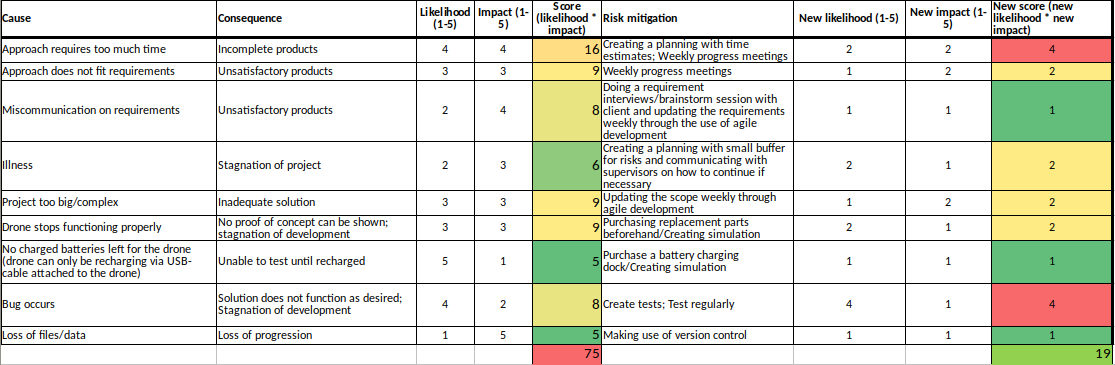
\includegraphics[width=\linewidth, angle=-90]{img/risk_matrix_post_midterm}
	\label{fig:risk_matrix}
	\caption{Risk matrix containing the risks with their mitigation plans.}
\end{figure}

% Please add the following required packages to your document preamble:
% \usepackage{graphicx}
%\begin{table}[]
	%\centering
	%\resizebox{\textwidth}{!}{%
		%\begin{tabular}{l|l|l|l|l|l|l|l|l}
			%\textbf{Cause} & \textbf{Consequence} & \textbf{Likelihood (1-5)} & \textbf{Impact (1-5)} & \textbf{Score (likelihood * impact)} & \textbf{Mitigation plan} & \textbf{New likelihood} & \textbf{New impact} & \textbf{New score} \\ \hline
			%Approach requires too much time & Incomplete products & 4 & 4 & 16 & Creating a planning with time estimates; Weekly progress meetings & 2 & 2 & 4 \\ \hline
			%Approach does not fit requirements & Unsatisfactory products & 3 & 3 & 9 & Weekly progress meetings & 1 & 2 & 2 \\ \hline
			%Miscommunication on requirements & Unsatisfactory products & 2 & 4 & 8 & Doing a requirement interviews/brainstorm session with client and updating the requirements weekly through the use of agile development & 1 & 1 & 1 \\ \hline
			%Illness & Stagnation of project & 2 & 3 & 6 & Creating a planning with small buffer for risks and communicating with supervisors on how to continue if necessary & 2 & 1 & 2 \\ \hline
			%Project too big/complex & Inadequate solution & 3 & 3 & 9 & Updating the scope weekly through agile development & 1 & 2 & 2 \\ \hline
			%Drone stops functioning properly & No proof of concept can be shown; stagnation of development & 3 & 3 & 9 & Purchasing replacement parts beforehand/Creating simulation & 2 & 1 & 2 \\ \hline
			%No charged batteries left for the drone (drone can only be recharging via USB-cable attached to the drone) & Unable to test until recharged & 5 & 1 & 5 & Purchase a battery charging dock/Creating simulation & 1 & 1 & 1 \\ \hline
			%Bug occurs & Solution does not function as desired; Stagnation of development & 4 & 2 & 8 & Create tests; Test regularly & 4 & 1 & 4 \\ \hline
			%Loss of files/data & Loss of progression & 1 & 5 & 5 & Making use of version control & 1 & 1 & 1 \\ \hline
			%&  &  &  & TOTAL = 75 &  &  &  & TOTAL = 19
		%\end{tabular}%
	%}
	%\caption{Risk matrix containing the risks with their consequences, scores, mitigation plans, and mitigated scores.}
	%\label{tab:risk_matrix}
%\end{table}